\section{导论}



\begin{frame}[fragile]{提纲}
\begin{easylist} \easyitem
& 什么是信息检索
& 为什么学习信息检索
& 信息检索的主要内容
& 课程情况
\end{easylist}
\end{frame}


\section{什么是信息检索}

\begin{frame}[fragile]{Examples}
\begin{easylist} \easyitem
& Stephen Wolfram: 宇宙的本质是计算
\url{http://www.wolframalpha.com/}
\url{http://www.guokr.com/article/439770/}
\end{easylist}
\end{frame}


\begin{frame}[fragile]{Example: 通过百度检索中国国家主席}
\begin{figure}
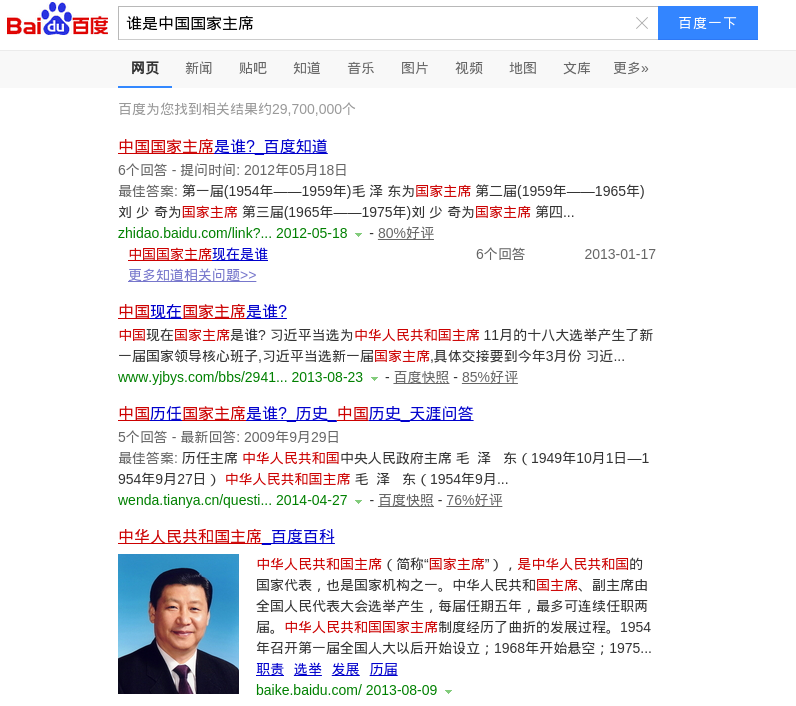
\includegraphics[scale=0.5]{figure/baidu-xijinping.png}
\end{figure}
\end{frame}


\begin{frame}[fragile]{Example: 通过Wolframalpha检索中国国家主席}
\begin{figure}
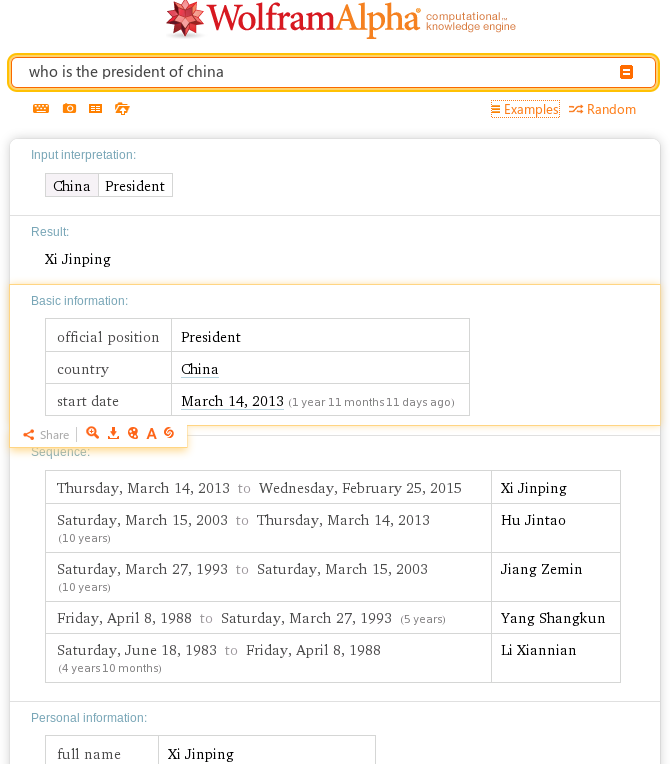
\includegraphics[scale=0.5]{figure/wolframalpha.png}
\end{figure}
\end{frame}


\begin{frame}[fragile]{信息检索}
\begin{easylist} \easyitem
& 信息检索:
&& 从大规模{\em 非结构化数据}(通常是文本)的集合中找出满足用户信息需求(Information Need)的资料(通常是文档)的过程。
    &&& 结构化数据
    &&& 非结构化数据
    &&& 半结构化数据
& 变化
&&  过去:图书馆管理员、律师助理、其他专业信息检索人员...
&& Web搜索引擎:信息检索取代关系数据库搜索成为信息访问的主要形式
&& 社会网络媒体: 用户通过与感兴趣的节点建立连接构建社会网络,借助于信息在网络中的扩散便可以实时获取相关信息,从而使社会媒体成为继搜索引擎之后的信息获取新途径。

\end{easylist}
\end{frame}


\begin{frame}[fragile]{历史}
\begin{easylist} \easyitem
& 20世纪40年代
&& 科学文献的大量涌现及计算机可用性的提高,引起了人们对自动检索的兴趣
&& 检索主要基于作者、标题和关键词进行
&& Calvin Mooers于1948年至1950年间提出了信息检索(Information Retrieval)这一术语
\end{easylist}

\infobox{Bush(1945):}{考虑一个供个人使用的未来设备,它是一种机械化的个人档案和图书馆。由于它需要一个名字,所以我随便造了一个名字叫memex。每个人可以将他所有的书、笔记或者他人的通信内容存储在memex上,它是一个机械化设备,能够提供快速灵活的查询功能。可以将他看成是对人记忆的补充。}
\end{frame}


\begin{frame}[fragile]{研究范围}
\begin{easylist} \easyitem
& 信息检索的全过程
& 用户对文档的浏览、过滤或对返回的文档进一步处理也属于信息检索的研究范畴,如:
&& 分类
&& 聚类
\end{easylist}
\end{frame}


\begin{frame}[fragile]{数据规模}
\begin{easylist} \easyitem
& 以Web搜索为代表的大规模级别
& 面向个人的小规模数据
&& Mac Spotlight...
& 面向企业、机构和特定领域的中等规模的检索
\end{easylist}
\end{frame}


\begin{frame}[fragile]{两种类型的用户检索任务}
\begin{easylist} \easyitem
& 特别检索(ad hoc retrieval)
&& 当查询提交给检索系统时,集合中的文档保持相对静止,是最常见的检索形式
& 过滤(Filtering)
&& 用户检索需求相对固定,而不断有新的文档进入系统。如新闻服务中,不断满足用户需求的文档反馈给用户。
&& 检索结果的排序不重要,重点在于如何构建描述用户信息需求的用户需求文档(User Profile)。
\end{easylist}
\end{frame}


\begin{frame}[fragile]{经典检索模型}
\begin{easylist} \easyitem
& 布尔模型
& 向量空间模型
& 概率模型
\end{easylist}
\end{frame}



\section{课程情况}
\begin{frame}[fragile]{课程介绍}
\begin{easylist} \easyitem
& 文本的表示
&& Local representations
&&& N-grams
&&& Bag-of-words
&&& 1-of-N coding

&& Continuous representations
&&& Latent Semantic Analysis
&&& Latent Dirichlet Allocation
&&& Distributed Representations
\end{easylist}
\end{frame}

\begin{frame}[fragile]{参考书}
\begin{easylist} \easyitem
& 信息检索导论
&& \url{http://nlp.stanford.edu/IR-book/} 
&& Christopher D. Manning, Prabhakar Raghavan and Hinrich Schütze, {\em Introduction to Information Retrieval }, Cambridge University Press. 2008.
& 刘挺等译, 搜索引擎——信息检索实践. 机械工业出版社, 2010.
& Reza Zafarani, Mohammad Ali Abbasi, Huan Liu, {\em Social Media Mining: An Introduction}, Cambridge University Press. 2014.
&& \url{http://dmml.asu.edu/smm/SMM.pdf}
& 王知津等译, Ricardo, 现代信息检索,机械工业出版社,2005.
& 夏立新等, 信息检索原理与技术,科学出版社,2009.
\end{easylist}
\end{frame}


\begin{frame}[fragile]{Paper/Slide}
\begin{easylist} \easyitem
& Slide:
&& Learning Representations of Text using Neural Networks
\end{easylist}
\end{frame}

\begin{frame}[fragile]{ ~ }
~~
\end{frame}

